\section{Условие}

\section{Теория}

Необходимо промоделировать систему, состоящую из генератора, памяти и
обслуживающего аппарата.

Генератор выдает сообщение распределенные по равномерному закону, они приходят в память и обрабатываются по нормальному закону, параметры задаются.

Необходимо определить оптимальную длину очереди, при которой не будет потерянных сообщений. Используя принципы $\Delta t$ и событий.

Как только определили выходной поток сообщений, задаваемую часть сообщений $A$ снова подаем в очередь.

\subsection{Событийный принцип}

Характерное свойство моделируемых систем – состояние отдельных устройств изменяется в дискретные моменты времени, которые совпадают с моментами поступления сообщений в систему, моментами окончания решения задач, моментами возникающих аварийных сигналов и т.д. Поэтому, моделирование и продвижение текущего времени в системе удобно проводить использую событийный принцип, при котором состояние всех блоков системы анализируется лишь в момент наступления какого-либо события. Момент наступления следующего события определяется минимальным значением из списка будущих событий, представляющих собой совокупность моментов ближайшего изменения состояний каждого из блоков системы.

\subsection{$\Delta t$ принцип}

Принцип $\Delta t$ заключается в последовательном анализе состояний всех блоков в момент $t + \Delta t$ по заданному состоянию блоков в момент $t$. При этом новое состояние блоков определяется в соответствии с их алгоритмическим описанием с учетом действующих случайных факторов, задаваемых распределениями вероятности. В результате такого анализа принимается решение о том, какие общесистемные события должны имитироваться программной моделью на данный момент времени.

Основной недостаток этого принципа: значительные затраты машинного времени на реализацию моделирования системы. А при недостаточно малом $\Delta t$ появляется опасность пропуска отдельных событий в системе, что исключает возможность получения адекватных результатов при моделировании.

Достоинство: равномерная протяжка времени.

\section{Результаты}

Ниже приведены результаты работы программы для обоих алгоритмов при разных значениях вероятности повторной заявки ($p$).

\begin{figure}[H]
    \centering
    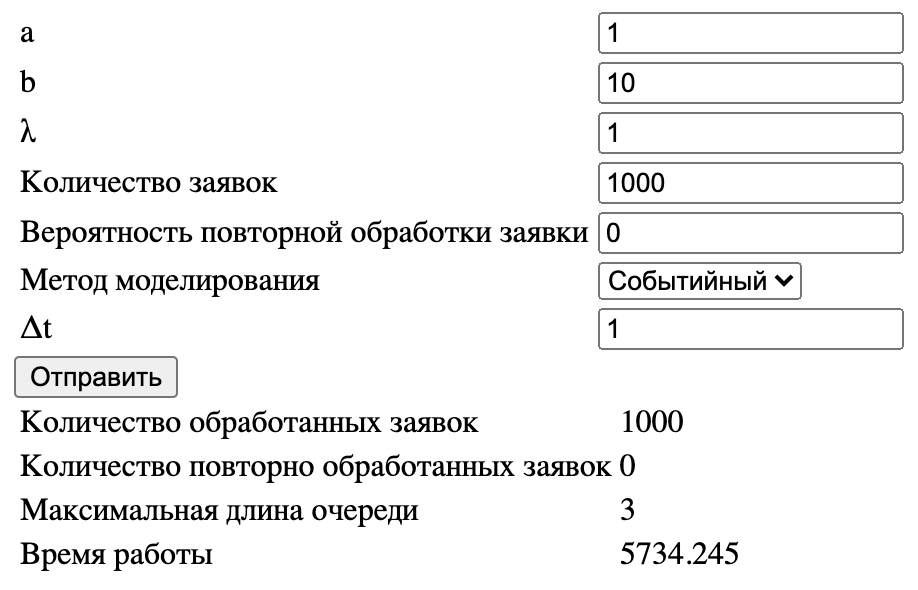
\includegraphics[width=0.6\textwidth]{img/content/event_0.png}
    \caption{Событийный метод, $p = 0$}
\end{figure}

\begin{figure}[H]
    \centering
    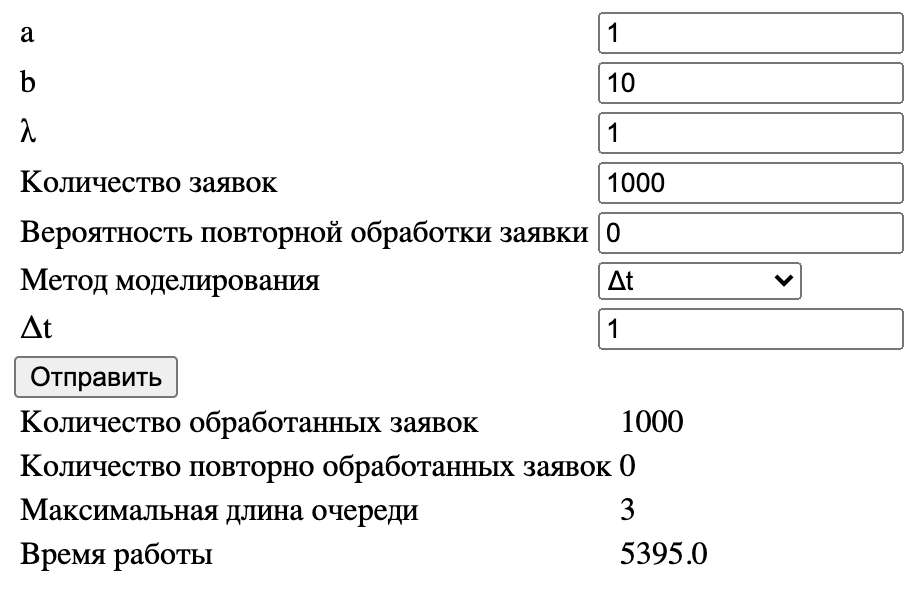
\includegraphics[width=0.6\textwidth]{img/content/dt_0.png}
    \caption{$\Delta t$ метод, $p = 0$}
\end{figure}

\begin{figure}[H]
    \centering
    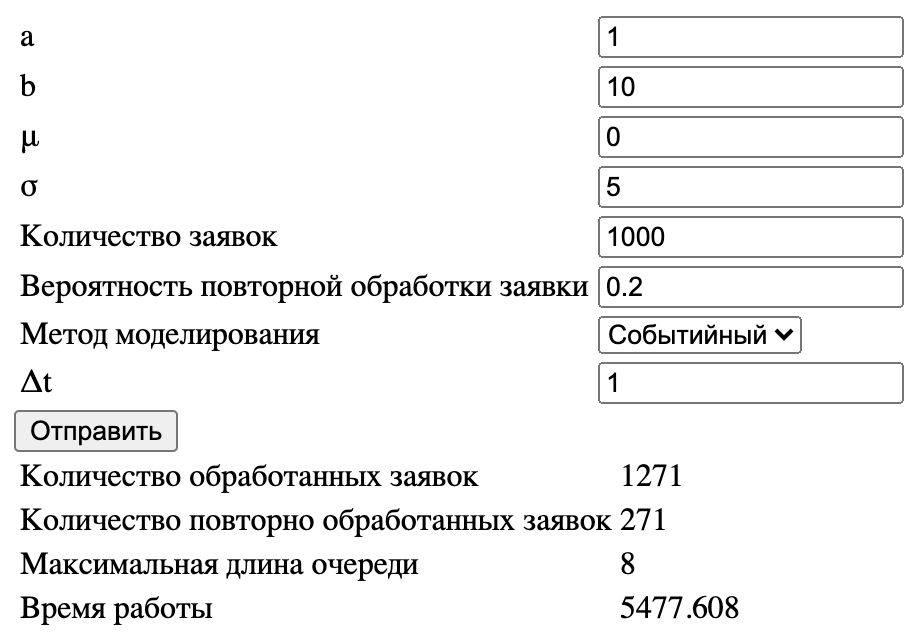
\includegraphics[width=0.6\textwidth]{img/content/event_2.png}
    \caption{Событийный метод, $p = 0.2$}
\end{figure}

\begin{figure}[H]
    \centering
    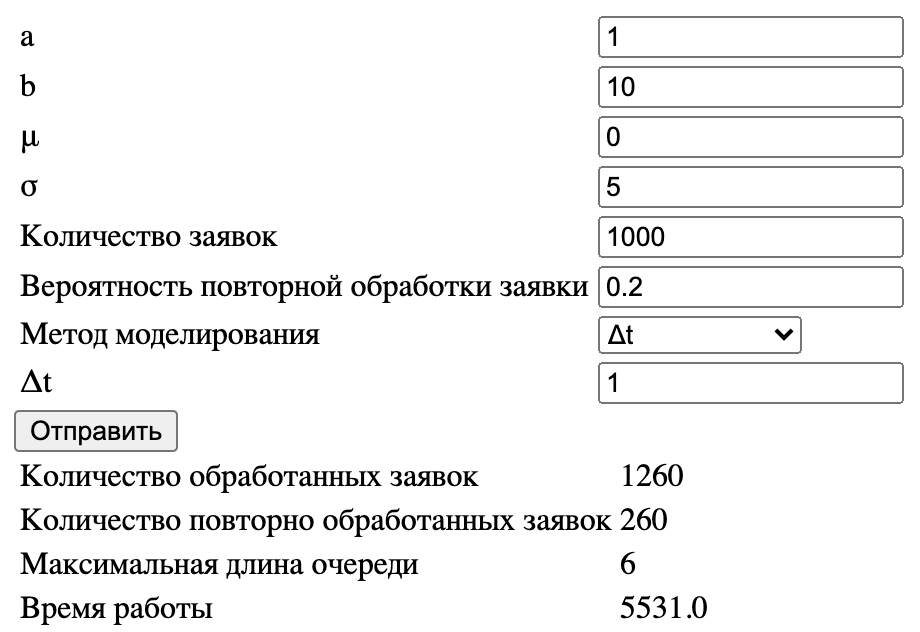
\includegraphics[width=0.6\textwidth]{img/content/dt_2.png}
    \caption{$\Delta t$ метод, $p = 0.2$}
\end{figure}

\begin{figure}[H]
    \centering
    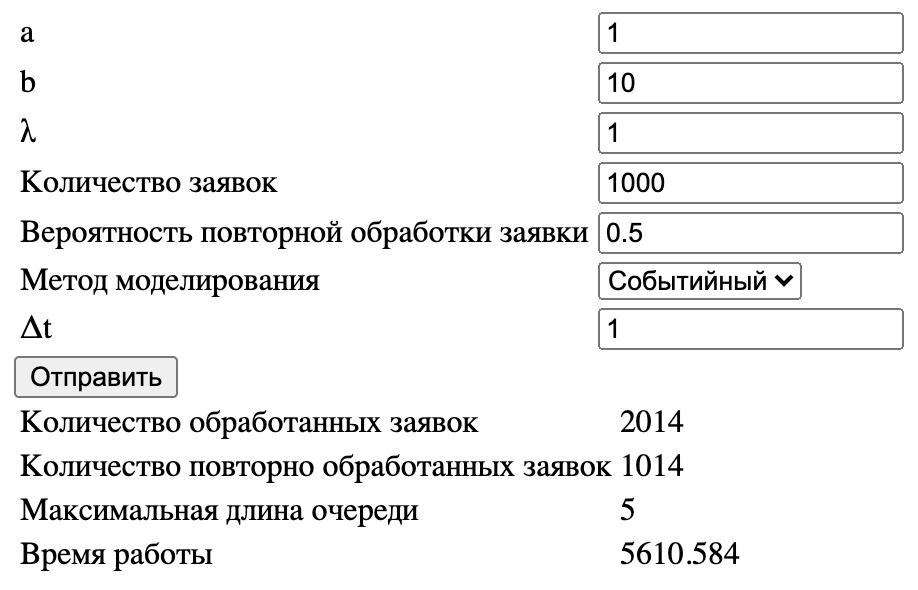
\includegraphics[width=0.6\textwidth]{img/content/event_5.png}
    \caption{Событийный метод, $p = 0.5$}
\end{figure}

\begin{figure}[H]
    \centering
    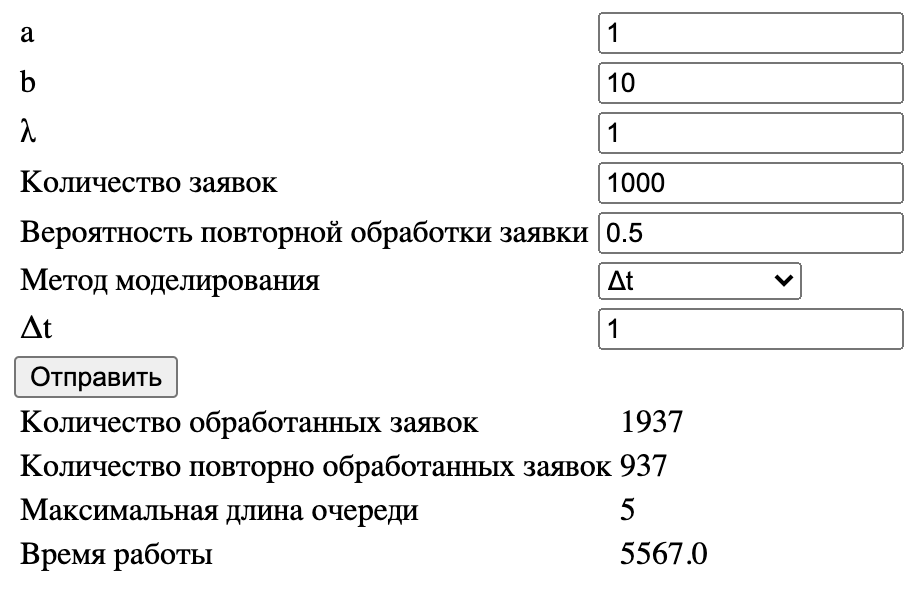
\includegraphics[width=0.6\textwidth]{img/content/dt_5.png}
    \caption{$\Delta t$ метод, $p = 0.5$}
\end{figure}

\begin{figure}[H]
    \centering
    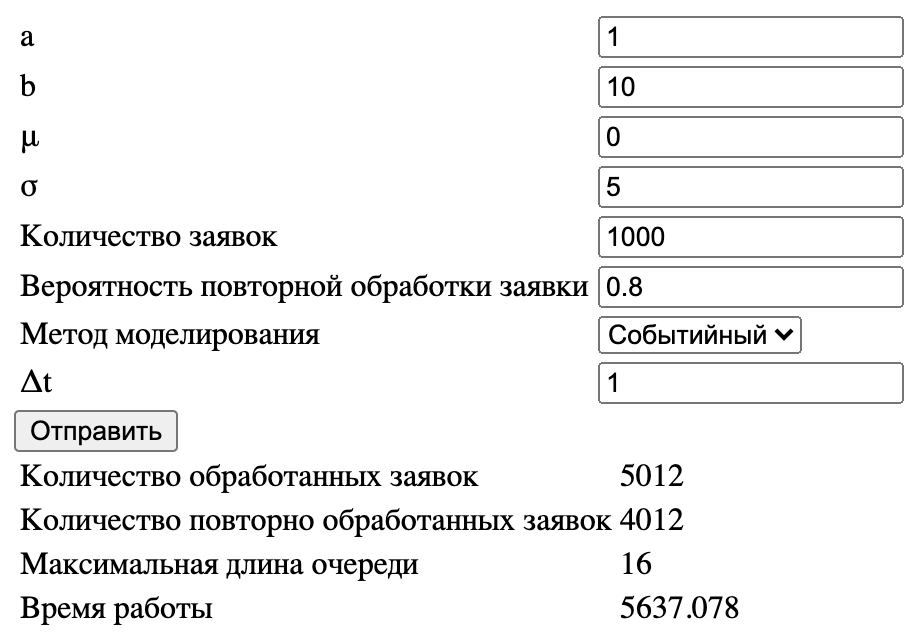
\includegraphics[width=0.6\textwidth]{img/content/event_8.png}
    \caption{Событийный метод, $p = 0.8$}
\end{figure}

\begin{figure}[H]
    \centering
    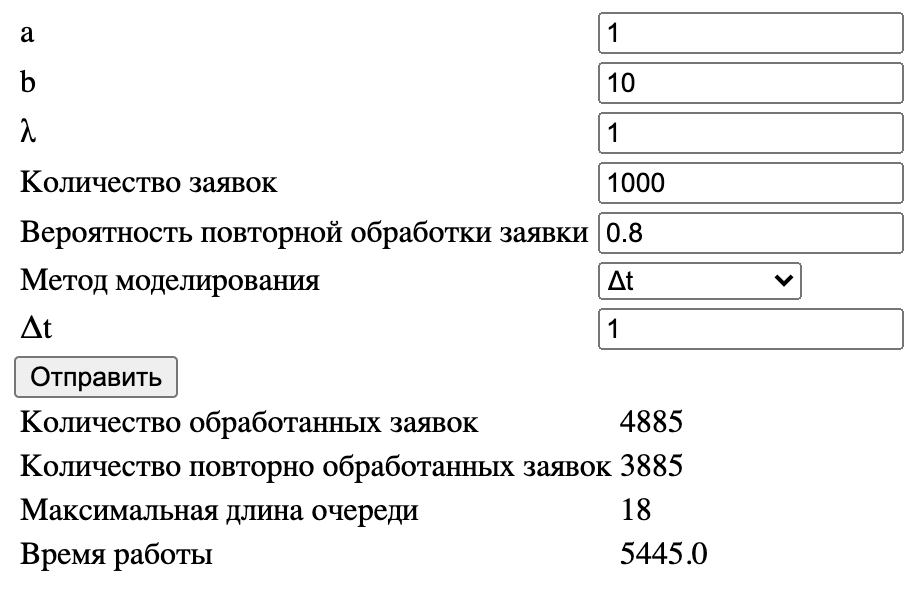
\includegraphics[width=0.6\textwidth]{img/content/dt_8.png}
    \caption{$\Delta t$ метод, $p = 0.8$}
\end{figure}

\begin{figure}[H]
    \centering
    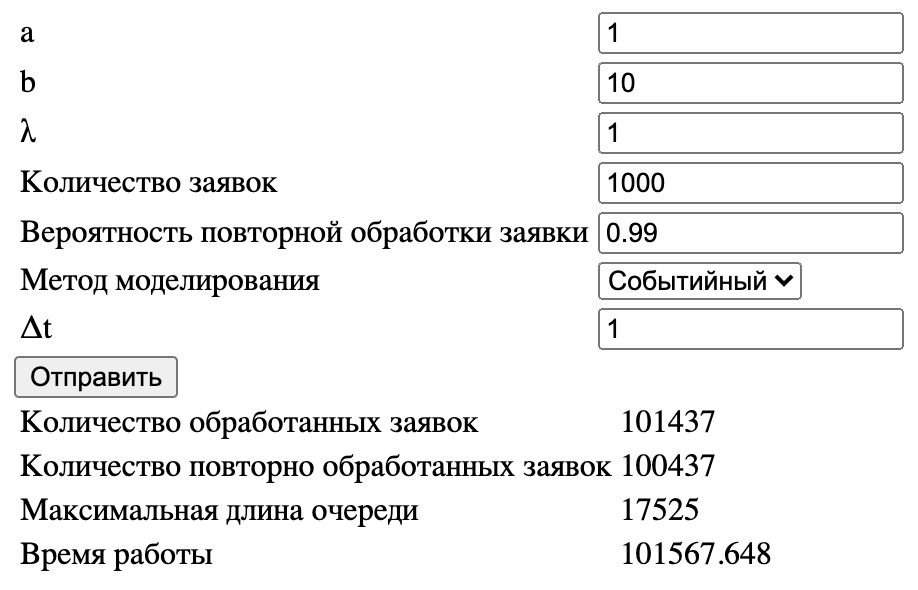
\includegraphics[width=0.6\textwidth]{img/content/event_99.png}
    \caption{Событийный метод, $p = 0.99$}
\end{figure}

\begin{figure}[H]
    \centering
    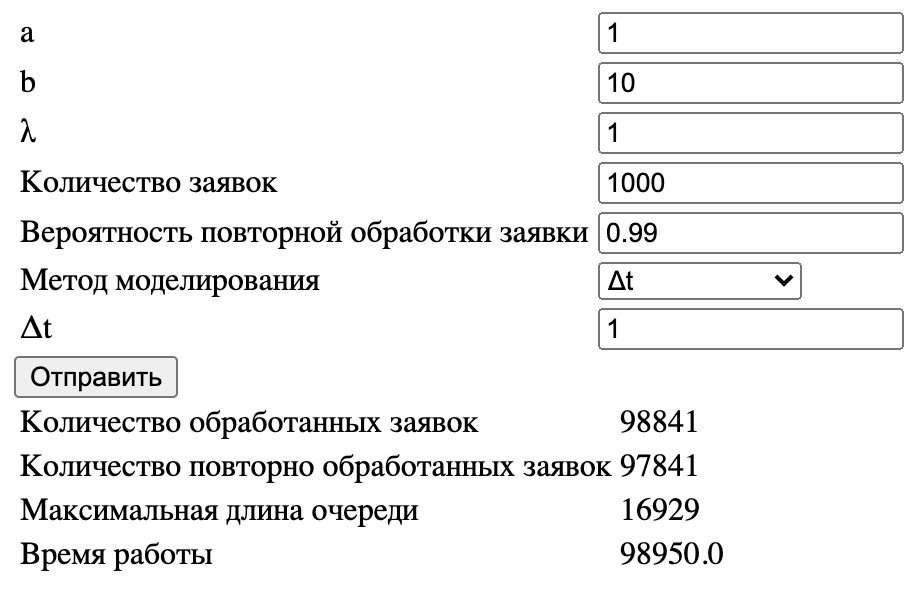
\includegraphics[width=0.6\textwidth]{img/content/dt_99.png}
    \caption{$\Delta t$ метод, $p = 0.99$}
\end{figure}

\section{Вывод}

Была смоделирована система, состоящая из генератора, памяти и обслуживающего аппарата.

На выходе была получена оптимальная длина очереди, число обработанных и повторно обработанных заявок, время обработки.
